\chapter{Estado del Arte del Browser} %buscar referencia
%LO EXISTENTE EN PAPERS, WEB, ETC. SOBRE EL TEMA DEÑ BROWSER!! MINIS-RESUMENES!!
\label{chap3:EA}

\section{Navegadores Existentes}
\label{chap3:BrowExis}

    \subsection{Google Chrome y Google Chromium}
    \label{chap3:GC}
    La misión de Google es organizar la información del mundo y lograr que sea útil y accesible para todo el mundo. Esta gran empresa partió como un búscador y rápidamente llegó a ser dueño de la mayor parte de búsquedas en el mundo. Tiene servicios de almacenamiento en la nube, correo electrónico, \textit{e-wallet} y otros más. Google ha sido responsable por la construcción del Navegador Web \textbf{Google Chrome} y \textit{Google Chromium}, siendo la segunda la versión open source.

    La arquitectura de Chrome o Chromium se basa principalmente en dos módulos: el Browser Kernel y el Rendering Engine, cómo se puede ver en la Figura \ref{fig:archG}.

    \begin{figure}[h!t]
        \begin{center}
            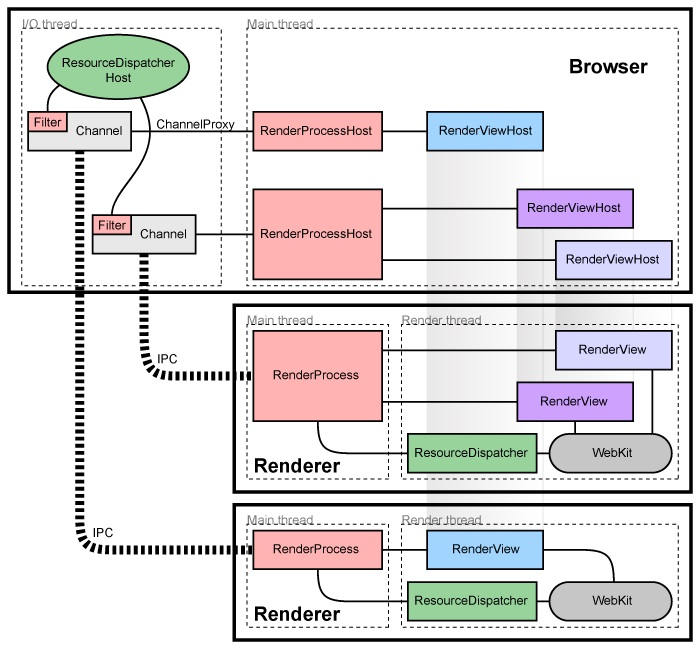
\includegraphics[scale=0.5]{figures/archGC.jpg}
          %\caption{Representación conceptual de una Nube con Eucalyptus. La especificación de las partes y su explicación se ve en \ref{sec:chap2.4.2}. Fuente \cite{EucalyptusOverview}}
          \label{fig:archG}
        \end{center}
    \end{figure}

    Én la documentación de Google Chromium \cite{multiProcArchG}, que es base para Google Chrome, afirma que la arquitectura soporta para cada tab un proceso nuevo, de manera de hacer al Browser más robusto y modularizar el sistema para evitar ciertas amenazas de seguridad. El proceso principal es llamado \textit{Browser Process/Kernel/Engine} y se encarga de la \textit{User Interface}, manejo de las tabs y los procesos de los \textit{plug-in}. Cada tab es asociado a un Rendering Engine, éstos tienen restricciones de acceso (\textit{Sandoboxing}) a los demas y al sistema, lo que permite que exista una protección de la memoria y un control de acceso. En \cite{barth2008security} se explica que el objetivo principal de esta arquitectura es poder mitigar ataques muy severos sin tener que sacrificar la compatibilidad con los sitios web ya existentes. Para lograr el objetivo Google ha ganado muchas lecciones de cómo realizar esto \cite{reis2009browser}, pues explican que un gran desafío en la seguridad es proteger a los usuarios de los atacantes que se aprovechan de las vulnerabilidades y debilidades de los clientes web-browsers. En su arquitectura modular se puede ver que se intenta proveer una seguridad que evita afectar la compatibilidad con otros sitios. La arquitectura comentada se basa en dos decisiones de diseño: La arquitectura depende en el Rendering Engine para aquellos componentes de alto riesgo como JavaScript, el parser de HTML y la creación de DOM para hacer cumplir SOP; al estar rodeados por un Sandboxing hace que el Rendering Engine se comporte como una caja negra. 


    Google Chrome expone en \cite{reis2009browser} que existen ciertas lecciones que han ido utilizando para mejorar la calidad de su browser. Estas son:

    \begin{itemize}
    	\item Reducción de las vulnerabilidades de seguridad, se basa en la aislación de ciertos componentes y la reducción de privilegios de ciertas tareas en el browser. La aislación lo lograron con la creación del Rendering Engine y el Browser Kernel, que tienen como objetivo proteger la data del sistema de archivos. Si bien esto puede no entregar muchos beneficios a una aplicación web, si lo hace en el usuario del browser.
    	\item Reducir la ventana de vulnerabilidades, la actualización del browser se hace cada cierto tiempo de forma automática para así cubrir las vulnerabilidades que van apareciendo.
    	\item Reducción de la frecuencia de exposición, Google trabaja con StopBadware.org para entregar una mayor seguridad al descubrir nuevos tipos de ataques y vulnerabilidades relacionadas con el browser.
    \end{itemize}



    \subsection{Internet Explorer}
    \label{chap3:IE}
    Internet Explorer es el navegador grafico predeterminado por Microsoft y que su primera versión 1.0 fue realizada en 1995. IE es una derivación de Spyglass Mosaic desarrolado por la NCSA (National Center for Supercomputing Applications). En primera instancia fue un navegador que podría ser obtebido si era comprado como complemento de \textit{Microsoft Plus!} o mediante la versión \textit{OEM} de Windows 95. Desde la tercera versión de IE, en 1996, que esta se lanzó de forma gratuita.
            
    La arquitectura de este navegador es modular y permite al desarrollador por utilizar los recursos para crear diferentes funcionalidades, ejemplo de esto son: toolbars, Microsoft Active X controls, etc. En la Figura \ref{fig:archIE} \cite{webpag3} se puede ver los principales componentes de la architectura del browser mencionado. IE utiliza \textit{COM} o \textit{Component Object Model} una interfaz binaria standard para componentes de software introducida por Microsoft en 1993 y que permite una comunicación entre procesos/componentes de software provenientes de la familia de software de Microsoft. \textit{COM} es similar a otras tecnologías de interfaz de componentes de software ( Component Software Interface Technologies) cómo CORBA y Java Beans. El uso de \textit{COM} gobierna la forma la interacción de los componentes que se comunicann y permite que haya un reuso y extensibilidad de estos.
            
    \begin{figure}[h!t]
        \begin{center}
    		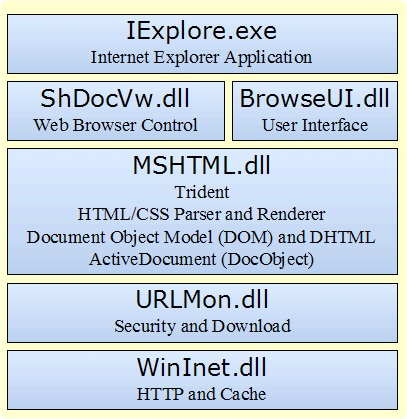
\includegraphics[scale=0.65]{figures/IEArch.jpg}
          %\caption{Representación conceptual de una Nube con Eucalyptus. La especificación de las partes y su explicación se ve en \ref{sec:chap2.4.2}. Fuente \cite{EucalyptusOverview}}
          \label{fig:archIE}
        \end{center}
    \end{figure}
      
    El ejecutable IExplore.exe es la base para el corazón del navegador \textit{Mshtml.dll} que se encarga del \textit{parsing} tanto de \textit{CSS} como del \textit{HTML} así como también de la función de renderizado de la página en el navegador; tiene también la tarea de alojar otros componentes dependiendo del contenido del HTML parseado, cómo JScript, XML Data, etc. Con codename \textit{Trident}, expone su interfaz para poder ser alojado por el componente \textit{Shdocvw.dll}, llamado también WebBrowser Control, que se encarga de poder dar funcionalidad, navigabilidad y un historial al browser, permitiendo que sea alojada facilmente en una \textit{Aplicación Windows}. La interfaz de usuario es proveída por \textit{Browsui.dll}. Cuando se realiza una descarga de un recurso, \textit{Urlmon.dll} pasa por una serie de pasos para asegurar que el tipo de archivo calce con el tipo \textit{MIME} declarado por el servidor. Finalmente, \textit{WinInet.dll} se encarga de implementar los protocolos de aplicación HTTP y FTP, agregando también el manejo del cache del browser.
            
    La arquitectura de Internet Explorer, basada en la tecnología \textbf{COM}, permite extender sus capacidade, por ejemplo: \textbf{Mediante Extensiones del browser}, \textbf{Extensiones de Contenido} y \textbf{Alojo y Reuso}.


    \subsection{Firefox}
    \label{chap3:Firefox}

    Firefox fue creado a partir del navegador \textit{Netscape} en 1998, actualmente la fundación Mozilla ha sido la que la ha mantenido, generando varias modificaciones desde su nacimiento. Las metas de diseño que Mozilla desee en el navegador son:
    \begin{itemize}
        \item Renderizado rápido de las páginas web.
        \item Fuerte apoyo a los estandares web como la W3C.
        \item Interoperabilidad en las diversas plataformas.
    \end{itemize}

    \begin{figure}[h!t]
        \begin{center}
    		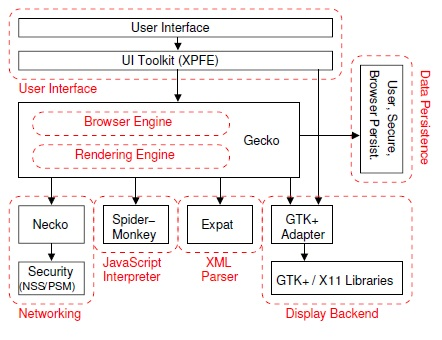
\includegraphics[scale=0.8]{figures/archMoz.jpg}
          %\caption{Representación conceptual de una Nube con Eucalyptus. La especificación de las partes y su explicación se ve en \ref{sec:chap2.4.2}. Fuente \cite{EucalyptusOverview}}
          \label{fig:archM}
        \end{center}
    \end{figure}
            
    La arquitectura de este browser puede ser vista en la Figura \ref{fig:archM} donde se pueden observar los siguientes componentes:
            \begin{itemize}
                \item La interfaz de usuario, puede ser reutilizada para otras aplicaciones.
                \item La persistencia de los datos, tanto de bookmarks como de data de bajo nivel como el \textit{cache}.
                \item EL \textit{Rendering Engine}, permite el renderizado de documentos HTML/XML aún cuando estos estén mal formados. Este Engine es capaz de renderizar la interfaz de la aplicación multi-plataforma.
            \end{itemize}
    La arquitectura de Mozilla se distingue de las demás en que la visualización especificada por la plataforma y la librería de \textit{widgets} son usados directamente en el navegador, lo que minimiza el costo necesario para soportar diferentes plataformas.
            




\section{Arquitectura de Referencia del Browser y Patrones}
\label{chap3:ArqRefBrowandPatt}
%Referirme a los artículos que hayan realizado antes el trabajo
%usar: 2005-grosskurth-browser-refarch, preprint-grosskurth-browser-archevol, webpag3 (IE), reis2009isolating

%Decir: "este trabajo es basado en la metodología de Fernandez \cite{Hashizume2014Reference} usando patrones en la construcción de la arquitectura de referencia"

La arquitectura de referencia a construir en este trabajo tiene como objetivo catalizar el entendimiento de la estrecha relación que existe entre el \cite{Web Browser} y los sistemas que serían construídos sobre la Internet. Éstas relaciones entre las dos entidades pueden llegar a ser bien importantes en los desarrollos de Software, pues puede explicar los posibles problemas que indirectamente sufre; considerar al Web browser como un \textit{concern} en el desarrollo de SW puede ser una buena estrategia para evitar una gran perdida monetaria u organizacional. Se sabe que el Browser es un pieza de Software que ha sufrido varios cambios desde la década de los 90, por lo tanto entre los desarrolladores de ésta herramienta ya existen conveniones de qué elementos funcionan mejor. Por consiguiente, no es de extrañar que diferentes browsers estén construidos de formas muy similares, y en consecuencia puedan ser conceptualizados en una Arquitectura de Referencia que manifeste los componentes, mecanismos de comunicación y funciones de esta pieza de Software.

El primer paso para realizar el estado del arte con respecto a este punto fue realizar una búsqueda ordenada y a través de string de búsqueda dentro de web engines y librerías digitales conocidas. Se utilizaron las siguientes plataformas para buscar documentación al respecto:
\begin{itemize}
    \item Google, usando ``google dorks'' para filtrar resultados
    \item Google Scholar, usando string de búsqueda y operadores booleanos para filtrar resultados.
    \item IEEE Xplore Digital Library, usando su buscador basado en comandos y utilizando operadores booleanos para filtrar (de buscó tanto en metadata como en el texto completo).
    \item Direct Science, CiteSeerX, Springer Link y otras librerías digitales. 
\end{itemize}

Para aquellos buscadores donde era posible usar operadores booleanos también se trató de filtrar el contenido para que pudiera mostrar resultados relacionados a: ``Browser'' y ``Reference Architecture''.

Sin embargo los resultados fueron bastante pobres. Desafortunadamente hasta la fecha no existe mucho trabajo relacionado a la construcción de una Arquitectura de Referencia para el Browser. Si bien existe un trabajo en concreto donde se plantea una Arquitectura de Referencia como el de \cite{2005-grosskurth-browser-refarch}, no se ha podido encontrar otros similiares. 


En el trabajo de \cite{2005-grosskurth-browser-refarch} se entrega la arquitectura de Referencia basada en el descubrimiento de las Arquitecturas concretas de los browser usados a través de herramientas de Ingeniería Inversa \textit{Reverse Engineering}. Sin embargo lo que relatan en el trabajo es algo que ya está muy desactualizado para los browsers modernos. 

En \cite{preprint-grosskurth-browser-archevol} se realiza una actualización del trabajo (un año después) pero enfocada a descubrir más arquitecturas concretas de otros web browser conocidos, en especial aquellos Open Source como: Konqueror, Lynx, Firefox, entre otros.


\section{Evolución y Seguridad en el Browser}
\label{chap3:EvoandSec}
%Usar referencias varga2013evolution, EvoBrowSecNSS, browSecPhish, browSecPrivSett, rowSecSEMBlock, silic2010security, barth2008security, reis2009browser, reis2009isolating, barth2009securing, barth2010protecting, Carlini12, liu2012chrome, utakrit2009review, barth2009secure, Accuvant11, Li12, Yu07, Zalewsk08, alcorn2014browser, sansInstInfoSec, 
% evolucion de la web: http://www.evolutionoftheweb.com/ (infografía)

En \cite{2005-grosskurth-browser-refarch} y \cite{preprint-grosskurth-browser-archevol} podemos notar que existe una mayor importancia en llegar a los componentes y las relaciones detrás del browser, y casi una nula mención de elementos de seguridad que permiten salvaguardar datos críticos o cómo protege al host de las amenazas. Podemos dar esta falta de conocimiento dado que en tales fehcas la cantidad de ataques de seguridad al Browser es mucho menos que en la actualidad %poner referencia.


\subsection{Estandarizaciones}
\label{chap3:Standars}

\subsection{Vulnerabilidades}
\label{chap3:vuln}

\subsection{Amenazas}
\label{chap3:threats}

\subsection{Medidas de Mitigación o Mecanismos de Defensa}
\label{chap3:mitig}

    \begin{enumerate}
        %CHROME/CHROMIUM
        \item Safe Browsing API and Content-Agnostic Malware Prevention
        \\XXX 
        %Lo usa chrome/chromium y FIREFOX!!!
        %Safe Browsing API es inefectiva contra ataques de Social Eng Malware, citas: rowSecSEMBlock
        %Abrams2013:    The NSS analyst brief, “Cybercrime  Kill    Chain   vs. Defense Effectiveness,” demonstrates    that    holes   in  one layer   of  defense are often   not  closed by  secondary   and tertiary technologies. Google   augments    its Safe    Browsing    API with    additional  download    protection  that    is  seven   times   more    effective   than    the Safe    Browsing    API.

        \item Sandoxing
        \\En el desarrollo de \cite{barth2008security} se define un modelo de amenazas donde se enumeran las habilidades que debería de tener un atacante y los objetivos de estos, para así caracterizar y evaluar las propiedades de seguridad necesarias para evitar que los atacantes cumplan su objetivo. Una propiedad importante que hacen destacar en el estudio es cómo aislar ciertos procesos que pueden ser aprovechados por los atacantes y ofrece una forma para poder mitigar esto: Sandboxing. El Sandboxing de Google Chrome previene al atacante de leer o escribir en el sistema de archivos del usuario, dejando al Principal Web con los privilegios necesarios para parsear un HTML/XML y ejecutar código JavaScript. Sin embargo esta arquitectura no imposibilita al atacante a atacar otros sitios web si es que el Rendering Engine fue comprometido, lo que puede convertirse en una amenaza muy grande para otros sitios web.

        \item Actualizaciones Periódicas en Background
        \\XXX

        \item Privacy Settings: Do Not Track and Third-Party Cookies
        \\XXX
        %En los 3 browsers


        %IE
        \item SmartScreen
        \\XXX
        
        \item Application Reputation / App Rep
        \\XXX


        %FIREFOX
        \item Content Security Policy
        \\XXX


        \item HTTP Headers
        \\XXX

    \end{enumerate}




\section{Sumario}
\label{chap3:Summ}